\documentclass[letterpaper, 12pt]{article}
\usepackage[margin=1in]{geometry}
\usepackage{amsmath}
\usepackage{amssymb}
\usepackage{fancyhdr}
%\usepackage{hyperref}
\usepackage{xcolor}
\usepackage{tikz}
\usepackage{pgfplots}
\usetikzlibrary{positioning, calc}
\setlength{\headheight}{15pt}

\pagestyle{fancy}
\fancyhf{}

\rhead{
    Shengdong Li
    Calc 1
}
\rfoot{
    Page \thepage
}

\usepackage{indentfirst}

\begin{document}
\title{Response to Grace Shang}
\author{by Shengdong Li}
\date{23 May 2020}
\maketitle

\section{Intro}
Hey Grace! Thank you so much for responding to my initial post! I'm amazed at your understanding of the physics/engineering topics and the connections that you drew, to the calculus that we learned in class, and your mentioning of the MVT, even though your initial post was all about statistics. \par
Below, I'll try to compare and contrast the differences in each of our justifications for the Arc Length formula, as well as explaining the $a$ and $b$ value better, as I should and could have explained that better.
\section{My way vs. Your way}
It seems to me that I had a more basic understanding of the justification of the arc length formula.
\begin{align}
\intertext{At the point where I had $\sqrt{dx^{2}+dy^{2}}$ for the length of the arc, instead of using the MVT, I rewrote the $dy$ as $f(b)-f(a)$, resulting in}
\sqrt{dx^{2}+\left(f\left(b\right)-f\left(a\right)\right)^{2}}
\intertext{When you multiply the numerator of a fraction with the same thing as the denominator, the fraction stays the same. So here, I multiplied the top and the bottom by $dx$.} 
\sqrt{dx^{2}+\left(\frac{f\left(b\right)-f\left(a\right)dx}{dx}\right)^{2}}
\intertext{Since $dy$ is $f(b)-f(a)$, naturally $dx$ is $b-a$. Plugging in $b-a$ for the value of $dx$ on the denominator gives us}
\frac{f\left(b\right)-f\left(a\right)}{b-a}dx. 
\intertext{$\frac{f\left(b\right)-f\left(a\right)}{b-a}$ is the definition of a derivative, and as such, we can replace it with $f'\left(x\right)$, resulting in }f'\left(x\right)dx
\intertext{Again, it's important to note here that $f'\left(x\right)dx$ still equals $dy$, since all we did to bring on this change was multiply by a fraction that equalled $1$. Therefore, we can plug this back into our original expression,$\sqrt{dx^{2}+dy^{2}}$, giving us}
\sqrt{dx^{2}+\left(f'\left(x\right)dx\right)^{2}}
\end{align}
...And an easy solve from there. \par
However, I like your way better, using the MVT, because (1) it is probably the official way to do it and (2) the MVT has a verified proof behind it while my way seems rather insufficient and is more of a proof of concept / justification than the MVT. \par
One very small issue or rather interesting note that I had with the MVT is the verbal definition. The verbal definition for the MVT, off the top of my head, is that if a function is continuious, if a secant line is draw from one point to another then within those points there must be a tangent line with the same slope as the secant line. Maybe I'm trolling, but the word definition of the MVT doesn't slot into this problem nearly as well. \par
Overall though, I was really impressed that you thought of using MVT in this problem, as it was something that I learned and forgot for the test and only remembered existed at this moment.
\section{Better explanation for arc lengths}
After reading about your confusion with the $a$ and $b$ values I realize that in the initial Arc Lengths lesson I didn't provide a lot of context for those values, and I apologize for that. Below, I tried make some overall improvements to the entire lesson, add some explanations for the $a$ and $b$ values, as well as update the triangle to account for them. I hope that this helps a bit!
\section{Arc Lengths}
The idea of finding the arc length of a function is based off looking at lengths of small segments in the function and adding it up together, like most other formulas in calclulus. \par
First, imagine that a function is made up of a bunch of points connected together.
\begin{center}
    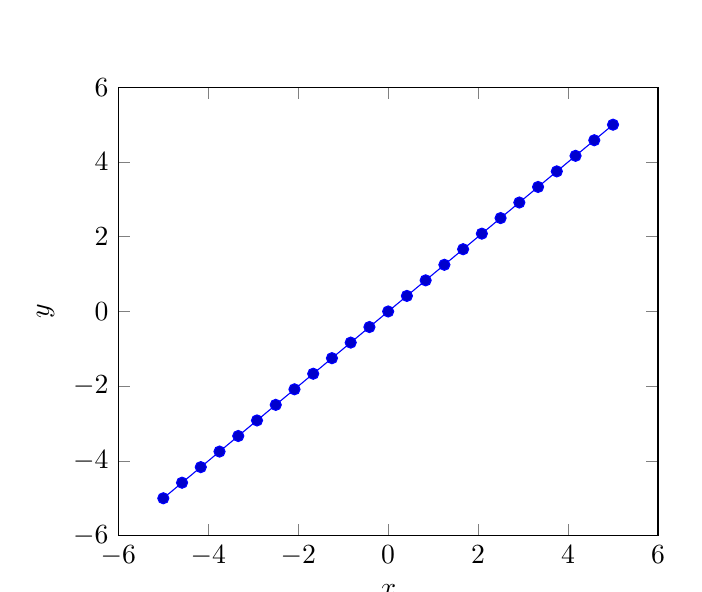
\begin{tikzpicture}
        \begin{axis}[
                xlabel=$x$,
                ylabel={$y$}
            ]
            % use TeX as calculator:
            \addplot {x};
        \end{axis}
    \end{tikzpicture}
\end{center}
If you zoom in on one of these segments with two points, you'll find that you can draw a triangle, imagining that the hypotenuse is the arc length, one leg is $dx$, and the other is $dy$. \par
You can then use the pythagorean theorem to calculate the arc length of this segment, a concept similar to the distance formula.
\begin{center}
    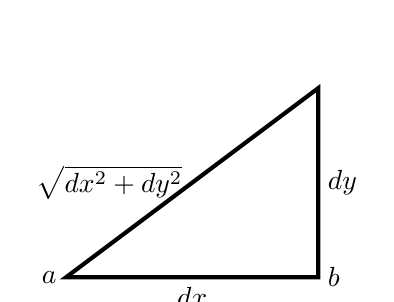
\begin{tikzpicture}[scale=0.8]
        % draw the background
        %\draw [line width=1.5pt, fill=gray!2] (0,0) -- (60:4) -- (4,0) -- cycle;

        \coordinate[label=left:$a$]  (A) at (0,0);
        \coordinate[label=right:$b$] (B) at (4,0);
        \coordinate[label=above:$$] (C) at (4,3);

        \coordinate[label=below:$dx$](c) at ($ (A)!.5!(B) $);
        \coordinate[label=left:$\sqrt{dx^2+dy^2}$](b) at ($ (A)!.5!(C) $);
        \coordinate[label=right:$dy$](a) at ($ (B)!.5!(C) $);

        %angle alpha
        %\draw[fill=red!30] (0,0) -- (0:0.75cm) arc (0:36.87:.75cm);
        %\draw (1cm,0.35cm) node {$\theta$};

        % angle beta
        %\begin{scope}[shift={(4cm,0cm)}]
        %    \draw[fill=green!30] (0,0) -- (-180:0.75cm) arc (180:120:0.75cm);
        %    \draw (150:0.5cm) node {$\beta$};
        %\end{scope}

        % angle gamma
        %\begin{scope}[shift={(60:4)}]
        %    \draw[fill=green!30] (0,0) -- (-120:.75cm) arc (-120:-60:.75cm);
        %    \draw (-90:0.5cm) node {$\gamma$};
        %\end{scope}

        % the triangle
        \draw [line width=1.5pt] (A) -- (B) -- (C) -- cycle;
    \end{tikzpicture}
\end{center}
(Above, the $x$ value of the left point is $a$ and the $x$ value of the right point is $b$.)
Now we just have to find the infinite sum of all of the small lengths combined from a starting point to an end point, which would look a little something like $\int_{a}^{b}\sqrt{dx^{2}+dy^{2}}$. However, we can't have both $dx$ and $dy$ in one problem, so let's work on $dy$ and try to make it in terms of $dx$. \par
$dy$ can be rewritten as $f(b)-f(a)$. Now, to produce the $dx$, let's rewrite this expression with $dx$ divided and multiplied, which would look like this: $\frac{f\left(b\right)-f\left(a\right)}{dx}\cdot dx$ and $dx$ can be written as $b-a$. Doing that for the denominator of the fraction would result in $\frac{f\left(b\right)-f\left(a\right)}{b-a}\cdot dx$. The fraction on the left is the definition of a derivative, so this entire thing can then be rewritten as $f'\left(x\right)dx$. \par
Pluggin this into our total arc length would result in $\int_{a}^{b}\sqrt{dx^{2}+\left(f'\left(x\right)dx\right)^{2}}$. Now we can use some algebra to clean this up a bit.
\begin{align}
    \int_{a}^{b}\sqrt{dx^{2}+\left(f'\left(x\right)dx\right)^{2}} & =\int_{a}^{b}\sqrt{dx^{2}\left(1+f'\left(x\right)^{2}\right)} \\
                                                                  & =\boxed{\int_{a}^{b}\sqrt{1+f'\left(x\right)^{2}}dx}
\end{align}
Which is the final arc length formula.
\section{Conclusion}
Thanks for responding to my post, reminding me of the MVT, and giving me some constructive feedback, Grace!\bigskip \par
Cheers,\par
Andy Li
\end{document}